% !TEX root = ../main.tex
% !TEX program = xelatex

\chapter{相关工作}\label{cha:related_work}
本章将重点介绍现有的刻画过程模型行为语义的算法(\ref{sec:related_algorithms}节),同时对本文改进的RORU算法进行介绍和分析(\ref{sec:roru}节)。

\section{过程模型行为语义刻画方法}\label{sec:related_algorithms}
国内外学者提出了诸多刻画过程模型行为语义的方法与工具,它们的适用场景和刻画能力各有不同。对过程模型行为语义的刻画可以应用到过程模型相似性度量方法及过程模型差异性检测中,本节重点介绍部分主流过程模型行为语义刻画方法和基于过程模型行为特征的相似性度量算法。

\subsection{变迁紧邻关系TAR}\label{subsec:tar}
Zha等人基于两个模型的变迁发生序列集提出了一种简单的相似性度量方法,即参考相似性算法(reference similarity)\cite{zha2010workflow}。作者同时给出了此方法的两个严重问题:首先,该方法不适用于带环模型,因为带环模型的变迁发生序列是无穷多的;其次,该方法过于严格,现实中存在发生序列相似但无完全相同序列的模型对,该类模型对会被认为完全不相似。

基于上述原因,Zha等人又提出了另一种相似性算法,即TAR算法(transition adjacency relation,变迁紧邻关系)。一对变迁$A,B$被认为是$TAR$集合中的元素当且仅当模型存在一条形如$\langle ...,A,B,...\rangle$的变迁发生序列,即变迁$A$后面紧跟着变迁$B$。令模型$M_{0}$和模型$M_{1}$的$TAR$关系集合分别是$TAR_{0}$和$TAR_{1}$,则两个模型间的$TAR$相似度被定义为$sim(M_{0},M_{1})=|TAR_{0}\cap TAR_{1}|/|TAR_{0}\cup TAR_{1}|$。因为模型$M_{0}$和$M_{1}$中的变迁数量是有限的,所以$TAR_{0}$和$TAR_{1}$是有穷的。作者同时证明了该算法对应的距离度量是度量空间中的距离函数。

TAR相似性算法解决了带环WF-net的相似性度量问题,是一种基于过程模型行为特征的相似性算法。但是TAR算法只考虑了变迁之间的直接紧邻关系,而忽略了变迁紧邻关系之间的传递闭包。该算法只考虑了“变迁$A$后可以被变迁$B$直接跟随”,而没有考虑“变迁$A$发生后,变迁$B$可以在之后某个时候发生”。该缺陷导致算法不能对循环结构与顺序结构对应的紧邻关系进行区分,影响度量结果。此外,TAR算法也不能正确处理带有非自由选择结构的过程模型。

\subsection{因果行为轮廓CBP}\label{subsec:cbp}
Weidlich等人通过抽取两个变迁执行之间的依赖关系刻画一个过程模型的行为语义\cite{weidlich2011efficient,weidlich2010efficient}。变迁之间的依赖关系被分成四类:
\begin{itemize}
  \item[-] 变迁$A$和变迁$B$满足严格顺序关系(strict order relation),当且仅当变迁$A$可能在变迁$B$之前被执行,而变迁$B$不可能在变迁$A$之前被执行,即存在形如$\langle ...A...B...\rangle$的变迁发生序列而不存在形如$\langle ...B...A...\rangle$的变迁发生序列。
  \item[-] 变迁$A$和变迁$B$满足互斥关系(exclusiveness relation),当且仅当变迁$A$和变迁$B$不可能在同一个变迁发生序列中同时出现。
  \item[-] 变迁$A$和变迁$B$满足观察并行关系(observation concurrency relation)(\onlinecite{weidlich2011efficient}中称之为交错顺序关系(interleaving order relation)),当且仅当变迁$A$可能在变迁$B$之前被执行,变迁$B$也可能在变迁$A$之前被执行。
  \item[-] 变迁$A$和变迁$B$满足共现关系(co-occurrence relation),当且仅当在每个变迁$A$出现的变迁发生序列中,变迁$B$也被执行。
\end{itemize}
上述四种关系被称为因果行为轮廓(causal behavioural profile,简称CBP)。

为了比较模型$M_{0}$和模型$M_{1}$的行为,首先需要为两个模型的变迁之间建立一个映射关系,该映射关系由一个相关关系$\sim$表示。关系$\sim$满足$M_{0}$可以与$M_{1}$的多个点对应,反之亦然。

Weidlich等人基于如下思想定义了一种相似性度量方法(\onlinecite{weidlich2011efficient,weidlich2010efficient}中称之为一致性程度):对于一个模型中每对变迁,如果在另一个模型中有对应的变迁对(由关系$\sim$决定),就检查这两个模型对是否满足相同的关系(严格顺序、互斥、交错顺序、共现)。

形式化的,令$T_{0}$和$T_{1}$分别为模型$M_{0}$和模型$M_{1}$的变迁集。定义$T_{0}^{\sim}=\{a\in T_{0}:\exists b\in T_{1},\text{s.t.}~a\sim b\}$以及$T_{1}^{\sim}=\{b\in T_{1}:\exists a\in T_{0},\text{s.t.}~a\sim b\}$。因为存在一对多的映射,所以$T_{0}^{\sim}$的大小与$T_{1}^{\sim}$不一定一致。一致性变迁对集合$C_{0}\subseteq T_{0}^{\sim}\times T_{0}^{\sim}$是所有满足如下条件的变迁对$(x_{0},y_{0})\in T_{0}^{\sim}\times T_{0}^{\sim}$:对于所有满足$x_{0}\sim x_{1}$且$y_{0}\sim y_{1}$的变迁对$(x_{1},y_{1})\in T_{1}^{\sim}\times T_{1}^{\sim}$,$x_{0}$和$y_{0}$有着与$x_{1}$和$y_{1}$相同的关系。同理定义一致性变迁对集合$C_{1}\subseteq T_{1}^{\sim}\times T_{1}^{\sim}$。

基于上述定义,可以用如下公式计算相似性(被称为一致性度量):
\begin{displaymath}
  sim(M_{0},M_{1})=\frac{\#C_{0}+\#C_{1}}{\#(T_{0}^{\sim}\times T_{0}^{\sim})+\#(T_{1}^{\sim}\times T_{1}^{\sim})}
\end{displaymath}

CBP可以被应用于模型检索和一致性检测。作者给出了一个高效计算过程模型因果行为轮廓的算法\cite{weidlich2010efficient},但该算法只适用于合理的自由选择WF-net。此外,在部分模型中,CBP不能区分循环结构和并行结构,所以拥有相同CBP的两个模型可能有着不同的行为。

\subsection{因果足迹CF}\label{subsec:cf}
Dijkman等人提出了因果足迹(causal footprints,简称CF)算法来抽取过程模型变迁之间的前驱关系\cite{dijkman2011similarity}。假定过程模型的变迁集合为$T$,它的因果足迹是一个二元组$(L_{lb},L_{la})$。该二元组的第一个元素$L_{lb}\subseteq (\wp(T)\times T)$被称为后向链接集合,$(S,a)\in L_{lb}$当且仅当在某个变迁发生序列中每次变迁$a$的发生都有变迁集合$S$中某个变迁的发生作为其前驱。同理,$L_{la}$被称为前向链接集合,$(T\times\wp(T))\supseteq(a,S)\in L_{la}$当且仅当在某个变迁发生序列中每次变迁$a$的发生都有变迁集合$S$中某个变迁的发生作为其后继。

为了度量两个模型间的相似性,需要计算它们的因果足迹之间的相似性。CF被当作文档向量空间中的文档,这是在信息过滤和信息检索领域中被广泛使用的一个概念\cite{salton1975vector}。因果足迹(“文档”)被表示成索引项的向量。假定模型$M_{0}=(N_{0},E_{0})$和$M_{1}=(N_{1},E_{1})$的前向链接集合分别为$L_{la}^{M_{0}}$和$L_{la}^{M_{1}}$,后向链接集合分别为$L_{lb}^{M_{0}}$和$L_{lb}^{M_{1}}$。索引项集合$\Uptheta=N_{0}\cup N_{1}\cup L_{la}^{M_{0}}\cup L_{la}^{M_{1}}\cup L_{lb}^{M_{0}}\cup L_{lb}^{M_{1}}$,即$\Uptheta$包含了两个模型的所有节点及所有的前向链接和后向链接。令$\lambda:\Uptheta\rightarrow\mathbb{N}$是一个索引函数,它给每个索引项赋予一个递增数字。

模型$M_{i}$($i\in\{0,1\}$)被表示成向量$\vec{g^{i}}=(g_{1}^{i},g_{2}^{i},...,g_{\#\Uptheta}^{i})$。\onlinecite{van2008measuring}给出了其取值:
\begin{displaymath}
  g{_{\lambda(t)}^i}=
    \begin{cases}
        0& if\quad t\notin N_i\cup L{_{la}^{M_i}}\cup L{_{lb}^{M_i}}\\
        1& if\quad t\in N_i\\
        \frac{1}{2^{len(t)}-1}& if\quad t\in L{_{la}^{M_i}}\cup L{_{lb}^{M_i}}
    \end{cases}
\end{displaymath}
其中$len(t)$是前向链接集合或者后向链接集合中元素的个数。模型$M_{0}$和模型$M_{1}$的相似度用两个模型的向量夹角余弦值表示:
\begin{displaymath}
  sim(M_{0},M_{1})=\frac{\vec{g^{0}}\cdot\vec{g^{1}}}{|\vec{g^{0}}|\cdot|\vec{g^{1}}|}
\end{displaymath}

CF的最大缺点在于$L_{la}$和$L_{lb}$含有大量的无用元素\cite{dijkman2011similarity,van2008measuring}。由于该方法使用的向量空间维度很高,因此向量的计算效率很低。另外,CF算法不区分$OR$连接和$XOR$连接,从而影响计算结果的合理性。

\subsection{主变迁序列PTS}\label{subsec:pts}
为了解决带环模型变迁发生序列集合无穷大的问题,Wang等人通过限制子序列来度量相似性:一条不含重复变迁的发生序列被看作一个整体来处理\cite{wang2010behavioral}。该算法被称为主变迁序列(principle transition sequences,简称PTS)。含有重复变迁$x$的序列$\sigma$被表达为$\sigma=\langle\sigma_{prefix},x,\sigma_{repeatable},x,...\rangle$,其中$\sigma_{prefix}$和$\sigma_{repeatable}$是$\sigma$的子序列。如此,在计算过程中,子序列$\sigma_{prefix}$和$\sigma_{repeatable}$会替代$\sigma$来参与计算。作者证明了对于每个过程模型,子序列的数量是有限的。

基于最长公共子序列可以定义两个子序列之间的相似性:
\begin{displaymath}
  sim_{trace}(\sigma_{1},\sigma_{2})=\frac{len(lcs(\sigma_{1},\sigma_{2}))}{max(len(\sigma_{1}),len(\sigma_{2}))}
\end{displaymath}
假定模型$M_{0}$和模型$M_{1}$的变迁集分别为$T_{0}$和$T_{1}$,基于上述子序列相似性可以得到模型相似性公式如下:
\begin{displaymath}
  sim(M_{0},M_{1})=\frac{\sum_{\sigma\in T_{0}}\text{max}_{\sigma'\in T_{1}}sim_{trace}(\sigma,\sigma')+\sum_{\sigma'\in T_{1}}\text{max}_{\sigma\in T_{0}}sim_{trace}(\sigma',\sigma)}{\#T_{0}+\#T_{1}}
\end{displaymath}

PTS算法对变迁发生序列集合的相似性计算较为粗糙,未考虑子序列基数差异的影响,且其只使用最大相似度来衡量集合间的相似性,计算结果不够精确。另一方面,当处理含有高并发结构的过程模型时,PTS算法存在状态空间爆炸的问题。

\subsection{完全触发序列集合CFS}\label{subsec:cfs}
作为对PTS算法的改进,Dong等人提出了基于触发序列集合的过程模型相似性算法,即CFS(全称complete firing sequences)\cite{dong2014cfs}。相比于PTS,CFS算法引入了循环计数的概念从而避免计算所有触发序列。CFS算法使用过程模型的覆盖树来计算触发序列集合,通过比较两个过程模型的触发序列集合来衡量两者的相似性。与PTS类似,作者首先定义了触发序列之间的相似性:
\begin{displaymath}
  sims(\sigma,\sigma')=\frac{length(lcs(L(\sigma),L(\sigma')))}{max(length(L(\sigma)),length(L(\sigma')))}
\end{displaymath}
在度量触发序列集合之间的相似性时,CFS不仅考虑了集合元素间的相似度,还考虑了两集合的基数差异。令$A$,$B$是两个完整触发序列集合,不失一般性假定$|A|\leq|B|$,令$\text{avg}(A,\sigma')=\frac{\sum_{\sigma\in A}sims(\sigma,\sigma')}{|A|}$表示完整触发序列集合$A$与单一完整触发序列$\sigma$的相似度,$\text{dis}(A,B)=\frac{||A|-|B||}{|B|}$表示$A$和$B$的基数距离。同时,令$M:A\rightarrow B$为一个单射,它将$A$中的完整触发序列映射到$B$中的序列,令$B'=B-\text{cod}(M)$,$n$为正整数,则$A$与$B$的相似度公式定义为:
\begin{displaymath}
  simc(A,B)=\frac{\sum_{(\sigma,\sigma')\in M}sims(\sigma,\sigma')+\sum_{\sigma'\in B'}\text{avg}(A,\sigma')}{|B|}\times(1-\frac{\text{dis}(A,B)}{n})
\end{displaymath}
并将此作为两个过程模型间的相似度。作者同时给出了利用贪心算法和$A^{*}$算法求解完整触发序列集合间最优映射的方法。与PTS类似,基于覆盖树的CFS算法也存在状态空间爆炸的问题。

\subsection{4C频谱}\label{subsec:4c}
Artem Polyvyanyy等人定义了Petri网的4C频谱(共现co-occurrence、冲突conflict、因果causality和并行concurrency)并据此刻画模型的行为语义\cite{polyvyanyy20144c}。作者首先探讨了冲突和共现关系,任意一种刻画变迁的发生之间关联情况的关系都可以被归纳成以下两种情况之一:两个变迁是否能在同一个发生序列中同时出现;一个变迁是否可以在某个其他变迁不发生的情况发生。基于此作者给出基本冲突和基本共现的定义:
\begin{definition}[基本冲突和基本共现]
令$S=(N=(P,T,F),M)$是一个标识Petri网,$x,y\in T$是其两个变迁。
  \begin{itemize}
    \item[-] $x$与$y$可以冲突,当且仅当$S$中存在一个变迁发生序列$\sigma$使得$x\in\sigma$且$y\notin\sigma$,记作$x\dashedrightarrow_{S}y$;
    \item[-] $x$与$y$可以共现,当且仅当$S$中存在一个变迁发生序列$\sigma$使得$x\in\sigma$且$y\in\sigma$,记作$x\leftrightharpoonupdown_{S}y$。\footnote{给定一个变迁发生序列$\sigma$,$x\in\sigma$表示$x$在$\sigma$中出现。}
  \end{itemize}
\end{definition}
在含义明确的情况脚标常被省略。借用析取范式和合取范式的概念作者进一步给出了4C频谱中的冲突和共现定义:
\begin{definition}[冲突和共现]
令$S=(N=(P,T,F),M)$是一个标识Petri网,$x,y\in T$是其两个变迁。
  \begin{itemize}
    \item[-] $x$与$y$共现,当且仅当$\overline{x\dashedrightarrow_{S}y}\wedge\overline{y\dashedrightarrow_{S}x}\wedge x\leftrightharpoonupdown_{S}y$,记作$x\leftrightarrow_{S}y$;
    \item[-] $x$与$y$冲突,当且仅当$x\dashedrightarrow_{S}y\wedge y\dashedrightarrow_{S}x\wedge\overline{x\leftrightharpoonupdown_{S}y}$,记作$x\#_{S}y$;
    \item[-] $x$需要$y$,当且仅当$\overline{x\dashedrightarrow_{S}y}\wedge y\dashedrightarrow_{S}x\wedge x\leftrightharpoonupdown_{S}y$,记作$x\rightharpoonup_{S}y$;
    \item[-] $x$与$y$相互独立,当且仅当$x\dashedrightarrow_{S}y\wedge y\dashedrightarrow_{S}x\wedge x\leftrightharpoonupdown_{S}y$,记作$x\rightleftharpoons_{S}y$。
  \end{itemize}
\end{definition}
除此之外还有两种与死变迁相关的合取范式:
\begin{definition}[不发生]
令$S=(N=(P,T,F),M)$是一个标识Petri网,$x,y\in T$是其两个变迁。
  \begin{itemize}
    \item[-] $x$与$y$从不发生,当且仅当$\overline{x\dashedrightarrow_{S}y}\wedge\overline{y\dashedrightarrow_{S}x}\wedge\overline{x\leftrightharpoonupdown_{S}y}$,记作$x\mid_{S}y$;
    \item[-] $x$发生但$y$不发生,当且仅当$x\dashedrightarrow_{S}y\wedge\overline{y\dashedrightarrow_{S}x}\wedge\overline{x\leftrightharpoonupdown_{S}y}$,记作$x\vdash_{S}y$。
  \end{itemize}
\end{definition}
综上得到冲突和共现关系的频谱:
\begin{definition}[冲突和共现关系的频谱]\label{def:spectrum_of_conflict_cooccurence}
令$S=(N=(P,T,F),M)$是一个标识Petri网,$x,y\in T$是其两个变迁。$\Omega$是一个由原子命题$x\dashedrightarrow_{S}y$、$y\dashedrightarrow_{S}x$和$x\leftrightharpoonupdown_{S}y$组成的命题范式。
  \begin{itemize}
    \item[-] $\Omega$描述$x$和$y$之间的冲突关系当且仅当$\Omega$的完美3DNF的每个合取范式含有$x\dashedrightarrow_{S}y$或者$y\dashedrightarrow_{S}x$;
    \item[-] $\Omega$描述$x$和$y$之间的共现关系当且仅当$\Omega$的完美3DNF的每个合取范式含有$x\leftrightharpoonupdown_{S}y$。
  \end{itemize}
\end{definition}
给定网$S$,分别用$\diamondtimes_{S}$和$\diamondplus_{S}$表示$S$中所有的冲突和共现关系。给定两个变迁$x$和$y$,共有四种合取范式包含了原子$x\leftrightharpoonupdown y$:(1)$x\dashedrightarrow y\wedge y\dashedrightarrow x\wedge x\leftrightharpoonupdown y$;(2)$\overline{x\dashedrightarrow y}\wedge y\dashedrightarrow x\wedge x\leftrightharpoonupdown y$;(3)$\overline{x\dashedrightarrow y}\wedge y\dashedrightarrow x\wedge x\leftrightharpoonupdown y$;(4)$\overline{x\dashedrightarrow y}\wedge\overline{y\dashedrightarrow x}\wedge x\leftrightharpoonupdown y$。因此,共有$2^{4}-1$,即15中不同的共现关系,每种共现关系都是一个或者多个上述合取范式的析取范式。同理,共有63种不同的冲突关系。

之后,作者开始探讨因果和并行关系。给定两个变迁$x$和$y$,对于因果和并行关系的分类建立在三个维度上:(1)关系是否在模型的部分或者全部过程流中成立;(2)关系是否在一个或者全部含有$x$的过程流中成立;(3)关系是否在一个或者全部含有$y$的过程流中成立。为了便于理解,首先给出一个能选择出描述$x$和$y$发生情况的过程流的过滤器:$\Delta_{S}(x,y)=\{\pi\in\Pi_{S}|\exists e_{1}\in E_{\pi}\exists e_{2}\in E_{\pi}:e_{1}\neq e_{2}\wedge\rho_{\pi}(e_{1})=x\wedge\rho_{\pi}(e_{2})=y\}$。为了检查两个变迁在所有包含它们的过程流中的并行模式,作者定义了完全并行关系。
\begin{definition}[完全并行]\label{def:total_concurrency}
令$S=(N=(P,T,F),M)$是一个标识Petri网,$x,y\in T$是其两个变迁。
  \begin{itemize}[leftmargin=22pt]
    \item[-] $x$和$y$满足完全(相互)并行关系,记作$x\parallel_{S}^{\forall\forall\forall}y$,当且仅当\\
    $
      \forall\pi\in\Delta_{S}(x,y)\forall e_{1}\in E_{\pi}\forall e_{2}\in E_{\pi}:(e_{1}\neq e_{2}\wedge\rho_{\pi}(e_{1})=x\wedge\rho_{\pi}(e_{2})=y)\Rightarrow e_{1}\parallel_{\pi}e_{2}
    $;
    \item[-] $x$对于$y$满足完全功能并行关系,记作$x\parallel_{S}^{\forall\forall\exists}y$,当且仅当\\
    $
      \forall\pi\in\Delta_{S}(x,y)\forall e_{1}\in E_{\pi}\exists e_{2}\in E_{\pi}:\rho(e_{1})=x\Rightarrow(\rho_{\pi}(e_{2})\wedge e_{1}\parallel_{\pi}e_{2})
    $;
    \item[-] $x$对于$y$满足完全支配并行关系,记作$x\parallel_{S}^{\forall\exists\forall}y$,当且仅当\\
    $
      \forall\pi\in\Delta_{S}(x,y)\exists e_{1}\in E_{\pi}\forall e_{2}\in E_{\pi}:\rho_{\pi}(e_{1})=x\wedge((\rho_{\pi}(e_{2})=y\wedge e_{1}\neq e_{2})\Rightarrow e_{1}\parallel_{\pi}e_{2})
    $;
    \item[-] $x$与$y$满足完全存在并行关系,记作$x\parallel_{S}^{\forall\exists\exists}y$,当且仅当\\
    $
      \forall\pi\in\Delta_{S}(x,y)\exists e_{1}\in E_{\pi}\exists e_{2}\in E_{\pi}:\rho_{\pi}(e_{1})=x\wedge\rho_{\pi}(e_{2})=y\wedge e_{1}\parallel_{\pi}e_{2}
    $。
  \end{itemize}
\end{definition}
为了检查两个变迁在至少一个包含它们的过程流中的并行模式,作者定义了存在并行关系。
\begin{definition}[存在并行]\label{def:existential_concurrency}
令$S=(N=(P,T,F),M)$是一个标识Petri网,$x,y\in T$是其两个变迁。
  \begin{itemize}[leftmargin=22pt]
    \item[-] $x$和$y$满足存在完全并行关系,记作$x\parallel_{S}^{\exists\forall\forall}y$,当且仅当\\
    $
      \exists\pi\in\Delta_{S}(x,y)\forall e_{1}\in E_{\pi}\forall e_{2}\in E_{\pi}:(e_{1}\neq e_{2}\wedge\rho_{\pi}(e_{1})=x\wedge\rho_{\pi}(e_{2})=y)\Rightarrow e_{1}\parallel_{\pi}e_{2}
    $;
    \item[-] $x$对于$y$满足存在功能并行关系,记作$x\parallel_{S}^{\exists\forall\exists}y$,当且仅当\\
    $
      \exists\pi\in\Delta_{S}(x,y)\forall e_{1}\in E_{\pi}\exists e_{2}\in E_{\pi}:\rho(e_{1})=x\Rightarrow(\rho_{\pi}(e_{2})\wedge e_{1}\parallel_{\pi}e_{2})
    $;
    \item[-] $x$对于$y$满足存在支配并行关系,记作$x\parallel_{S}^{\exists\exists\forall}y$,当且仅当\\
    $
      \exists\pi\in\Delta_{S}(x,y)\exists e_{1}\in E_{\pi}\forall e_{2}\in E_{\pi}:\rho_{\pi}(e_{1})=x\wedge((\rho_{\pi}(e_{2})=y\wedge e_{1}\neq e_{2})\Rightarrow e_{1}\parallel_{\pi}e_{2})
    $;
    \item[-] $x$与$y$满足存在(完全)并行关系,记作$x\parallel_{S}^{\exists\exists\exists}y$,当且仅当\\
    $
      \exists\pi\in\Delta_{S}(x,y)\exists e_{1}\in E_{\pi}\exists e_{2}\in E_{\pi}:\rho_{\pi}(e_{1})=x\wedge\rho_{\pi}(e_{2})=y\wedge e_{1}\parallel_{\pi}e_{2}
    $。
  \end{itemize}
\end{definition}
将定义\ref{def:total_concurrency}和定义\ref{def:existential_concurrency}中的$e_{1}\parallel_{\pi}e_{2}$替换成$e_{1}\rightarrowtail_{\pi}e_{2}$就得到了完全因果关系和存在因果关系的定义。

令$\Phi=\{\forall\forall\forall,\forall\forall\exists,\forall\exists\forall,\forall\exists\exists,\exists\forall\forall,\exists\forall\exists,\exists\exists\forall,\exists\exists\exists\}$,因果和并行关系的频谱定义如下:
\begin{definition}[因果和并行关系的频谱]\label{def:spectrum_of_causality_concurrency}
令$S=(N=(P,T,F),M)$是一个标识Petri网,$x,y\in T$是其两个变迁。
  \begin{itemize}
    \item[-] $x$和$y$满足因果关系,记作$x\rightarrowtail_{S,\diamonddot}^{\phi}y$,当且仅当\\
    $(x\diamonddot_{S}y)\wedge(x\rightarrowtail_{S}^{\phi}y)$,其中$\diamonddot_{S}\in\diamondplus_{S}$,$\phi\in\Phi$;
    \item[-] $x$和$y$满足并行关系,记作$x\parallel_{S,\diamonddot}^{\phi}y$,当且仅当\\
    $(x\diamonddot_{S}y)\wedge(x\parallel_{S}^{\phi}y)$,其中$\diamonddot_{S}\in\diamondplus_{S}$,$\phi\in\Phi$。
  \end{itemize}
\end{definition}
定义\ref{def:spectrum_of_causality_concurrency}可以推导出$15\times 8=120$中不同的因果关系和相同数量的并行关系。定义\ref{def:spectrum_of_conflict_cooccurence}和定义\ref{def:spectrum_of_causality_concurrency}共同组成了变迁之间行为关系的4C频谱。

4C频谱是一种完整且基本的关系定义,但是作者在\onlinecite{polyvyanyy20144c}中只给出了其中四种关系的计算方法。此外,存在两个拥有相同4C频谱关系但有着不同行为语义的模型\cite{armas2014suitability}。

\section{精炼不确定性有序关系}\label{sec:roru}
既然本文主要工作是对RORU算法的改进,有必要对\onlinecite{jin2014computing}中的RORU算法进行介绍。首先定义$\Sigma=(P,T,F,M_{0})$是标识Petri网,$\beta=(B,E,A,f)$是$\Sigma$的分支过程,$x,y,a,b,c\in E$都是$\beta$的事件。一条路径指分支过程中从开始状态到终止状态的一条有向路径。

基于一个任务是否总是和另一个任务在同一个执行实例中被执行,因果关系可以被精炼成以下四种。其中C是Certain的简写,U是Uncertain的简写。

\begin{definition}[确定-确定因果,简称C-C因果]\label{def:c_c_causal}
$x$和$y$满足C-C因果关系,记作$x\twoheadrightarrow y$,当且仅当:
  \begin{itemize}
    \item[-] $x$和$y$满足因果关系,即$x<y$;
    \item[-] 如果$x$出现在一条路径上,$y$必须之后也出现在这条路径上;
    \item[-] 如果$y$出现在一条路径上,$x$必须之前也出现在这条路径上。
  \end{itemize}
\end{definition}

\begin{definition}[确定-不确定因果,简称C-U因果]\label{def:c_u_causal}
$x$和$y$满足C-U因果关系,记作$x\rightharpoonup y$,当且仅当:
  \begin{itemize}
    \item[-] $x$和$y$满足因果关系,即$x<y$;
    \item[-] 如果$x$出现在一条路径上,$y$可能之后不出现在这条路径上;
    \item[-] 如果$y$出现在一条路径上,$x$必须之前也出现在这条路径上。
  \end{itemize}
\end{definition}

\begin{definition}[不确定-确定因果,简称U-C因果]\label{def:u_c_causal}
$x$和$y$满足U-C因果关系,记作$x\mapsto y$,当且仅当:
  \begin{itemize}
    \item[-] $x$和$y$满足因果关系,即$x<y$;
    \item[-] 如果$x$出现在一条路径上,$y$必须之后也出现在这条路径上;
    \item[-] 如果$y$出现在一条路径上,$x$可能之前不出现在这条路径上。
  \end{itemize}
\end{definition}

\begin{definition}[不确定-不确定因果,简称U-U因果]\label{def:u_u_causal}
$x$和$y$满足U-U因果关系,记作$x\rightleftharpoons y$,当且仅当:
  \begin{itemize}
    \item[-] $x$和$y$满足因果关系,即$x<y$;
    \item[-] 如果$x$出现在一条路径上,$y$可能之后不出现在这条路径上;
    \item[-] 如果$y$出现在一条路径上,$x$可能之前不出现在这条路径上。
  \end{itemize}
\end{definition}

类似地,可以将并行关系也精炼为以下四种。

\begin{definition}[确定-确定并行,简称C-C并行]\label{def:c_c_concurrency}
$x$和$y$满足C-C并行关系,记作$x\equiv y$,当且仅当:
  \begin{itemize}
    \item[-] $x$和$y$满足并行关系,即$x~co~y$;
    \item[-] 如果$x$被执行,$y$必须也在同一个实例中被执行;
    \item[-] 如果$y$被执行,$x$必须也在同一个实例中被执行。
  \end{itemize}
\end{definition}

\begin{definition}[确定-不确定并行,简称C-U并行]\label{def:c_u_concurrency}
$x$和$y$满足C-U并行关系,记作$x\Downarrow y$,当且仅当:
  \begin{itemize}
    \item[-] $x$和$y$满足并行关系,即$x~co~y$;
    \item[-] 如果$x$被执行,$y$可能不在同一个实例中被执行;
    \item[-] 如果$y$被执行,$x$必须也在同一个实例中被执行。
  \end{itemize}
\end{definition}

\begin{definition}[不确定-确定并行,简称U-C并行]\label{def:u_c_concurrency}
$x$和$y$满足U-C并行关系,记作$x\Uparrow y$,当且仅当:
  \begin{itemize}
    \item[-] $x$和$y$满足并行关系,即$x~co~y$;
    \item[-] 如果$x$被执行,$y$必须也在同一个实例中被执行;
    \item[-] 如果$y$被执行,$x$可能不在同一个实例中被执行。
  \end{itemize}
\end{definition}

\begin{definition}[不确定-不确定并行,简称U-U并行]\label{def:u_u_concurrency}
$x$和$y$满足U-U并行关系,记作$x\Updownarrow y$,当且仅当:
  \begin{itemize}
    \item[-] $x$和$y$满足并行关系,即$x~co~y$;
    \item[-] 如果$x$被执行,$y$可能不在同一个实例中被执行;
    \item[-] 如果$y$被执行,$x$可能不在同一个实例中被执行。
  \end{itemize}
\end{definition}

之后,作者提出一些用于紧邻任务计算的基本规则和用于非紧邻任务计算的传递性规则,并基于此给出了一个基于CPU计算无环过程模型RORU的算法。RORU有着一些明显的缺点,不能被应用于实际企业中。

首先,RORU不能被应用于带环的WF-net,这已经在\onlinecite{jin2014computing}的标题中明确指出。其次,由于RORU没有考虑不可见变迁,变迁发生序列中的发生顺序紧邻但模型结构上不紧邻的变迁无法被区分,所以两个有着不同行为语义的WF-net可能会被混淆。例如,图\ref{fig:sda_example_1}中WF-net的变迁发生序列集合是$\{\langle I,A,B,O\rangle,\langle I,B,A,O\rangle,\langle I,A,O\rangle,\langle I,B,O\rangle\}$而图\ref{fig:sda_example_2}中WF-net的变迁发生序列集合是$\{\langle I,A,B,O\rangle,\langle I,B,A,O\rangle,\langle I,A,O\rangle,\langle I,B,O\rangle,\langle I,O\rangle\}$。显然,这两个WF-net的行为是不一致的,但是RORU不能区分它们。

\begin{figure}[htbp]
  \centering
  \begin{subfigure}[b]{0.45\textwidth}
    \centering
    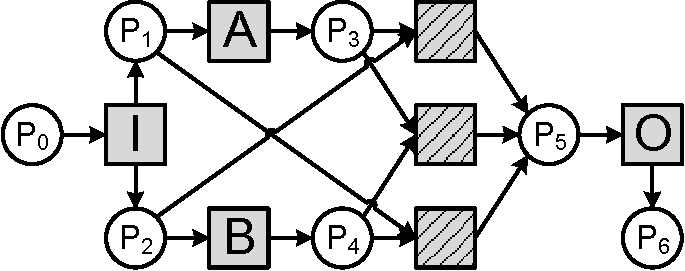
\includegraphics[width=1\textwidth]{sda_example_1}
    \caption{\label{fig:sda_example_1}}
  \end{subfigure}
  \hspace{1em}
  \begin{subfigure}[b]{0.45\textwidth}
    \centering
    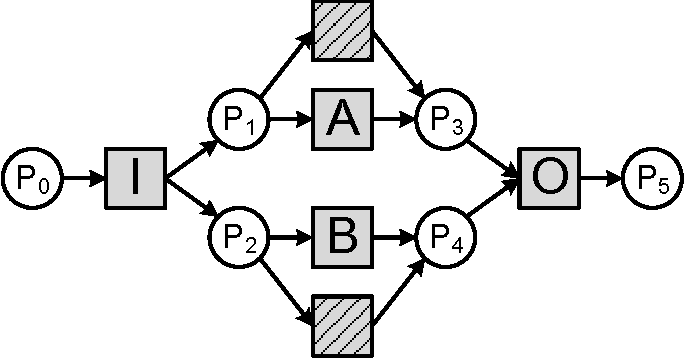
\includegraphics[width=1\textwidth]{sda_example_2}
    \caption{\label{fig:sda_example_2}}
  \end{subfigure}
  \vspace{6pt}
  \caption{RORU无法区分的一对含有不可见变迁的模型}
  \label{fig:sda_example}
\end{figure}

在一个含有非自由选择结构\cite{de2003workflow}的WF-net中,变迁之间的因果关系不一定满足传递性。以图\ref{fig:nfc_example_1}和图\ref{fig:nfc_example_2}中的模型为例,变迁$A$和变迁$C$满足因果关系,变迁$C$和变迁$E$亦满足因果关系。根据RORU的传递性规则,变迁$A$和变迁$E$应满足因果关系。然而,这在图\ref{fig:nfc_example_1}含有非自由选择结构的WF-net中是不正确的,因为当变迁$A$首先被执行后,只有变迁$C$和变迁$D$(而不是变迁$E$)可以被执行。因此,变迁$A$和变迁$E$永远不会满足因果关系。

\begin{figure}[htbp]
  \centering
  \begin{subfigure}[b]{0.45\textwidth}
    \centering
    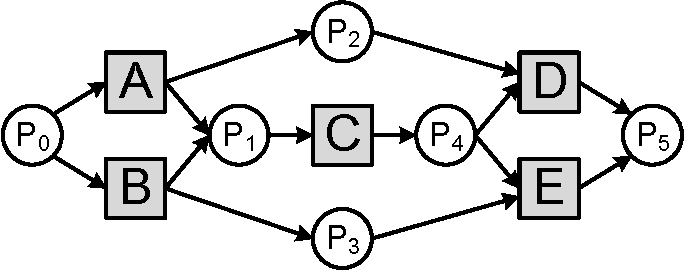
\includegraphics[width=1\textwidth]{nfc_example_1}
    \caption{\label{fig:nfc_example_1}}
  \end{subfigure}
  \hspace{1em}
  \begin{subfigure}[b]{0.45\textwidth}
    \centering
    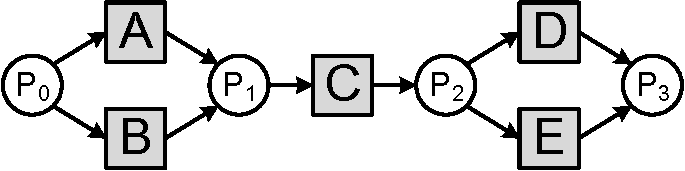
\includegraphics[width=1\textwidth]{nfc_example_2}
    \caption{\label{fig:nfc_example_2}}
  \end{subfigure}
  \vspace{6pt}
  \caption{RORU无法区分的一对含有非自由选择结构的模型}
  \label{fig:nfc_example}
\end{figure}

为了解决上述RORU存在的问题,本文将RORU中的有序关系进一步扩展,从而得到一个更为精细的方法去区分任意两个过程模型的行为语义。除了细化原算法的不确定性概念之外,本文引入了任务间多关系的概念,即一对任务之间可能含有不止一种关系。多关系概念的引入可以检测两个过程模型间更为细微的差异。

\section{本章小结}
本章首先对过程模型行为语义刻画算法的国内外研究现状进行了简要介绍和分析,选取了TAR、BP、CF、PTS、CFS、4C等算法为例并分析了它们的优缺点。本章随后对本文工作的基础RORU算法进行了详细的介绍并探讨了其缺陷。